\pdfbookmark{Общая характеристика работы}{characteristic}             % Закладка pdf
\section*{Общая характеристика работы}

\newcommand{\actuality}{\pdfbookmark[1]{Актуальность}{actuality}\underline{\textbf{\actualityTXT}}}
\newcommand{\progress}{\pdfbookmark[1]{Разработанность темы}{progress}\underline{\textbf{\progressTXT}}}
\newcommand{\aim}{\pdfbookmark[1]{Цели}{aim}\underline{{\textbf\aimTXT}}}
\newcommand{\tasks}{\pdfbookmark[1]{Задачи}{tasks}\underline{\textbf{\tasksTXT}}}
\newcommand{\aimtasks}{\pdfbookmark[1]{Цели и задачи}{aimtasks}\aimtasksTXT}
\newcommand{\novelty}{\pdfbookmark[1]{Научная новизна}{novelty}\underline{\textbf{\noveltyTXT}}}
\newcommand{\influence}{\pdfbookmark[1]{Практическая значимость}{influence}\underline{\textbf{\influenceTXT}}}
\newcommand{\methods}{\pdfbookmark[1]{Методология и методы исследования}{methods}\underline{\textbf{\methodsTXT}}}
\newcommand{\defpositions}{\pdfbookmark[1]{Положения, выносимые на защиту}{defpositions}\underline{\textbf{\defpositionsTXT}}}
\newcommand{\reliability}{\pdfbookmark[1]{Достоверность}{reliability}\underline{\textbf{\reliabilityTXT}}}
\newcommand{\probation}{\pdfbookmark[1]{Апробация}{probation}\underline{\textbf{\probationTXT}}}
\newcommand{\contribution}{\pdfbookmark[1]{Личный вклад}{contribution}\underline{\textbf{\contributionTXT}}}
\newcommand{\publications}{\pdfbookmark[1]{Публикации}{publications}\underline{\textbf{\publicationsTXT}}}


{\actuality} Обзор, введение в тему, обозначение места данной работы в
мировых исследованиях и~т.\:п., можно использовать ссылки на~другие
работы~\autocite{Gosele1999161,Lermontov}
(если их~нет, то~в~автореферате
автоматически пропадёт раздел <<Список литературы>>). Внимание! Ссылки
на~другие работы в~разделе общей характеристики работы можно
использовать только при использовании \verb!biblatex! (из-за технических
ограничений \verb!bibtex8!. Это связано с тем, что одна
и~та~же~характеристика используются и~в~тексте диссертации, и в
автореферате. В~последнем, согласно ГОСТ, должен присутствовать список
работ автора по~теме диссертации, а~\verb!bibtex8! не~умеет выводить в~одном
файле два списка литературы).
При использовании \verb!biblatex! возможно использование исключительно
в~автореферате подстрочных ссылок
для других работ командой \verb!\autocite!, а~также цитирование
собственных работ командой \verb!\cite!. Для этого в~файле
\verb!common/setup.tex! необходимо присвоить положительное значение
счётчику \verb!\setcounter{usefootcite}{1}!.

Для генерации содержимого титульного листа автореферата, диссертации
и~презентации используются данные из файла \verb!common/data.tex!. Если,
например, вы меняете название диссертации, то оно автоматически
появится в~итоговых файлах после очередного запуска \LaTeX. Согласно
ГОСТ 7.0.11-2011 <<5.1.1 Титульный лист является первой страницей
диссертации, служит источником информации, необходимой для обработки и
поиска документа>>. Наличие логотипа организации на~титульном листе
упрощает обработку и~поиск, для этого разметите логотип вашей
организации в папке images в~формате PDF (лучше найти его в векторном
варианте, чтобы он хорошо смотрелся при печати) под именем
\verb!logo.pdf!. Настроить размер изображения с логотипом можно
в~соответствующих местах файлов \verb!title.tex!  отдельно для
диссертации и автореферата. Если вам логотип не~нужен, то просто
удалите файл с~логотипом.

\ifsynopsis
Этот абзац появляется только в~автореферате.
Для формирования блоков, которые будут обрабатываться только в~автореферате,
заведена проверка условия \verb!\!\verb!ifsynopsis!.
Значение условия задаётся в~основном файле документа (\verb!synopsis.tex! для
автореферата).
\else
Этот абзац появляется только в~диссертации.
Через проверку условия \verb!\!\verb!ifsynopsis!, задаваемого в~основном файле
документа (\verb!dissertation.tex! для диссертации), можно сделать новую
команду, обеспечивающую появление цитаты в~диссертации, но~не~в~автореферате.
\fi

% {\progress}
% Этот раздел должен быть отдельным структурным элементом по
% ГОСТ, но он, как правило, включается в описание актуальности
% темы. Нужен он отдельным структурынм элемементом или нет ---
% смотрите другие диссертации вашего совета, скорее всего не нужен.

{\aim} данной работы является \ldots

Для~достижения поставленной цели необходимо было решить следующие {\tasks}:
\begin{enumerate}[beginpenalty=10000] % https://tex.stackexchange.com/a/476052/104425
  \item Исследовать, разработать, вычислить и~т.\:д. и~т.\:п.
  \item Исследовать, разработать, вычислить и~т.\:д. и~т.\:п.
  \item Исследовать, разработать, вычислить и~т.\:д. и~т.\:п.
  \item Исследовать, разработать, вычислить и~т.\:д. и~т.\:п.
\end{enumerate}


{\novelty}
\begin{enumerate}[beginpenalty=10000] % https://tex.stackexchange.com/a/476052/104425
  \item Впервые \ldots
  \item Впервые \ldots
  \item Было выполнено оригинальное исследование \ldots
\end{enumerate}

{\influence} \ldots

{\methods} \ldots

{\defpositions}
\begin{enumerate}[beginpenalty=10000] % https://tex.stackexchange.com/a/476052/104425
  \item Разработка метода настройки оптического интерферометра с использованеием методов машинного обучения с подкреплением
  \item Реализация метода автоматической растройки оптического интерферометра в виде программно-аппаратного комплекса
  \item Разработка иерархического агента для игры Nethack
\end{enumerate}
В папке Documents можно ознакомиться с решением совета из Томского~ГУ
(в~файле \verb+Def_positions.pdf+), где обоснованно даются рекомендации
по~формулировкам защищаемых положений.

{\reliability} полученных результатов обеспечивается \ldots \ Результаты находятся в соответствии с результатами, полученными другими авторами.


{\probation}
Основные результаты работы докладывались~на:
перечисление основных конференций, симпозиумов и~т.\:п.

{\contribution} Автор принимал активное участие \ldots

\ifnumequal{\value{bibliosel}}{0}
{%%% Встроенная реализация с загрузкой файла через движок bibtex8. (При желании, внутри можно использовать обычные ссылки, наподобие `\cite{vakbib1,vakbib2}`).
    {\publications} Основные результаты по теме диссертации изложены
    в~XX~печатных изданиях,
    X из которых изданы в журналах, рекомендованных ВАК,
    X "--- в тезисах докладов.
}%
{%%% Реализация пакетом biblatex через движок biber
    \begin{refsection}[bl-author, bl-registered]
        % Это refsection=1.
        % Процитированные здесь работы:
        %  * подсчитываются, для автоматического составления фразы "Основные результаты ..."
        %  * попадают в авторскую библиографию, при usefootcite==0 и стиле `\insertbiblioauthor` или `\insertbiblioauthorgrouped`
        %  * нумеруются там в зависимости от порядка команд `\printbibliography` в этом разделе.
        %  * при использовании `\insertbiblioauthorgrouped`, порядок команд `\printbibliography` в нём должен быть тем же (см. biblio/biblatex.tex)
        %
        % Невидимый библиографический список для подсчёта количества публикаций:
        \printbibliography[heading=nobibheading, section=1, env=countauthorvak,          keyword=biblioauthorvak]%
        \printbibliography[heading=nobibheading, section=1, env=countauthorwos,          keyword=biblioauthorwos]%
        \printbibliography[heading=nobibheading, section=1, env=countauthorscopus,       keyword=biblioauthorscopus]%
        \printbibliography[heading=nobibheading, section=1, env=countauthorconf,         keyword=biblioauthorconf]%
        \printbibliography[heading=nobibheading, section=1, env=countauthorother,        keyword=biblioauthorother]%
        \printbibliography[heading=nobibheading, section=1, env=countregistered,         keyword=biblioregistered]%
        \printbibliography[heading=nobibheading, section=1, env=countauthorpatent,       keyword=biblioauthorpatent]%
        \printbibliography[heading=nobibheading, section=1, env=countauthorprogram,      keyword=biblioauthorprogram]%
        \printbibliography[heading=nobibheading, section=1, env=countauthor,             keyword=biblioauthor]%
        \printbibliography[heading=nobibheading, section=1, env=countauthorvakscopuswos, filter=vakscopuswos]%
        \printbibliography[heading=nobibheading, section=1, env=countauthorscopuswos,    filter=scopuswos]%
        %
        \nocite{*}%
        %
        {\publications} Основные результаты по теме диссертации изложены в~\arabic{citeauthor}~печатных изданиях,
        \arabic{citeauthorvak} из которых изданы в журналах, рекомендованных ВАК\sloppy%
        \ifnum \value{citeauthorscopuswos}>0%
            , \arabic{citeauthorscopuswos} "--- в~периодических научных журналах, индексируемых Web of~Science и Scopus\sloppy%
        \fi%
        \ifnum \value{citeauthorconf}>0%
            , \arabic{citeauthorconf} "--- в~тезисах докладов.
        \else%
            .
        \fi%
        \ifnum \value{citeregistered}=1%
            \ifnum \value{citeauthorpatent}=1%
                Зарегистрирован \arabic{citeauthorpatent} патент.
            \fi%
            \ifnum \value{citeauthorprogram}=1%
                Зарегистрирована \arabic{citeauthorprogram} программа для ЭВМ.
            \fi%
        \fi%
        \ifnum \value{citeregistered}>1%
            Зарегистрированы\ %
            \ifnum \value{citeauthorpatent}>0%
            \formbytotal{citeauthorpatent}{патент}{}{а}{}\sloppy%
            \ifnum \value{citeauthorprogram}=0 . \else \ и~\fi%
            \fi%
            \ifnum \value{citeauthorprogram}>0%
            \formbytotal{citeauthorprogram}{программ}{а}{ы}{} для ЭВМ.
            \fi%
        \fi%
        % К публикациям, в которых излагаются основные научные результаты диссертации на соискание учёной
        % степени, в рецензируемых изданиях приравниваются патенты на изобретения, патенты (свидетельства) на
        % полезную модель, патенты на промышленный образец, патенты на селекционные достижения, свидетельства
        % на программу для электронных вычислительных машин, базу данных, топологию интегральных микросхем,
        % зарегистрированные в установленном порядке.(в ред. Постановления Правительства РФ от 21.04.2016 N 335)
    \end{refsection}%
    \begin{refsection}[bl-author, bl-registered]
        % Это refsection=2.
        % Процитированные здесь работы:
        %  * попадают в авторскую библиографию, при usefootcite==0 и стиле `\insertbiblioauthorimportant`.
        %  * ни на что не влияют в противном случае
        \nocite{vakbib2}%vak
        \nocite{patbib1}%patent
        \nocite{progbib1}%program
        \nocite{bib1}%other
        \nocite{confbib1}%conf
    \end{refsection}%
        %
        % Всё, что вне этих двух refsection, это refsection=0,
        %  * для диссертации - это нормальные ссылки, попадающие в обычную библиографию
        %  * для автореферата:
        %     * при usefootcite==0, ссылка корректно сработает только для источника из `external.bib`. Для своих работ --- напечатает "[0]" (и даже Warning не вылезет).
        %     * при usefootcite==1, ссылка сработает нормально. В авторской библиографии будут только процитированные в refsection=0 работы.
}

При использовании пакета \verb!biblatex! будут подсчитаны все работы, добавленные
в файл \verb!biblio/author.bib!. Для правильного подсчёта работ в~различных
системах цитирования требуется использовать поля:
\begin{itemize}
        \item \texttt{authorvak} если публикация индексирована ВАК,
        \item \texttt{authorscopus} если публикация индексирована Scopus,
        \item \texttt{authorwos} если публикация индексирована Web of Science,
        \item \texttt{authorconf} для докладов конференций,
        \item \texttt{authorpatent} для патентов,
        \item \texttt{authorprogram} для зарегистрированных программ для ЭВМ,
        \item \texttt{authorother} для других публикаций.
\end{itemize}
Для подсчёта используются счётчики:
\begin{itemize}
        \item \texttt{citeauthorvak} для работ, индексируемых ВАК,
        \item \texttt{citeauthorscopus} для работ, индексируемых Scopus,
        \item \texttt{citeauthorwos} для работ, индексируемых Web of Science,
        \item \texttt{citeauthorvakscopuswos} для работ, индексируемых одной из трёх баз,
        \item \texttt{citeauthorscopuswos} для работ, индексируемых Scopus или Web of~Science,
        \item \texttt{citeauthorconf} для докладов на конференциях,
        \item \texttt{citeauthorother} для остальных работ,
        \item \texttt{citeauthorpatent} для патентов,
        \item \texttt{citeauthorprogram} для зарегистрированных программ для ЭВМ,
        \item \texttt{citeauthor} для суммарного количества работ.
\end{itemize}
% Счётчик \texttt{citeexternal} используется для подсчёта процитированных публикаций;
% \texttt{citeregistered} "--- для подсчёта суммарного количества патентов и программ для ЭВМ.

Для добавления в список публикаций автора работ, которые не были процитированы в
автореферате, требуется их~перечислить с использованием команды \verb!\nocite! в
\verb!Synopsis/content.tex!.
 % Характеристика работы по структуре во введении и в автореферате не отличается (ГОСТ Р 7.0.11, пункты 5.3.1 и 9.2.1), потому её загружаем из одного и того же внешнего файла, предварительно задав форму выделения некоторым параметрам

Диссертационная работа была выполнена при поддержке гранта УМНИК № 120ГУЦЭС8-D3/56352 от 21.12.2019. 

%\underline{\textbf{Объем и структура работы.}} Диссертация состоит из~введения,
%четырех глав, заключения и~приложения. Полный объем диссертации
%\textbf{ХХХ}~страниц текста с~\textbf{ХХ}~рисунками и~5~таблицами. Список
%литературы содержит \textbf{ХХX}~наименование.

\pdfbookmark{Содержание работы}{description}                          % Закладка pdf
\section*{Содержание работы}
Во \underline{\textbf{введении}} обосновывается актуальность
исследований, проводимых в~рамках данной диссертационной работы. Приводится обзор литературы показывающий большой потенциал методов машинного обучения с подкреплением в задачах связанных с принятием решений. Формулируется цель и ставятся задачи данной работы. Излагается научная новизна
и практическая значимость научных результатов представляемой работы. 
В~последующих главах сначала описывается общий принцип, работы методов машинного обучения с подкреплением. Затем рассматриваются современные методы машинного обучения с подкреплением позволяющие достигать наилучших результатов в тестовых задачах. Потом приводится описание задачи настройки оптического интерферометра в виде задачи машинного обучения с подкреплением. Приводятся результаты обучения модели в симуляции и последующего тестирования разработанной модели на экспериментальной установке. В следующей главе формулируется необходимость в сложных тестовых задачах для развития и тестирования обобщающей способности методов машинного обучения с подкреплением. Формулируются отличительные особенности позволяющие считать среду, основанную на игре Nethack одной из самых сложных тестовых сред для алгоритмов машинного обучения с подкреплением. Затем приводится разработанный алгоритм для этой задачи и анализируется качество его работы. В заключении суммируются основные результаты, полученные в рамках подготовки диссертационного исследования с указанием их новизны и практической значимости. 


\underline{\textbf{Первая глава}} посвящена обзору методов машинного обучения с подкреплением (RL) и применению их в роботике. В ней формулируется задача RL - максимизация математического ожидания суммарной дисконтированной награды при взаимодействии RL агента со средой. Схематически это взаимодействие изображено на рисунке \ref{fig:rl_setting}. На рисунке \ref{fig:rl_setting} агент взаимодействует со средой по средством действий (action) и получает от среды следующее состояние, награду и флаг завершения эпизода (state, reward, done).

\begin{figure}[ht]
    \centerfloat{
        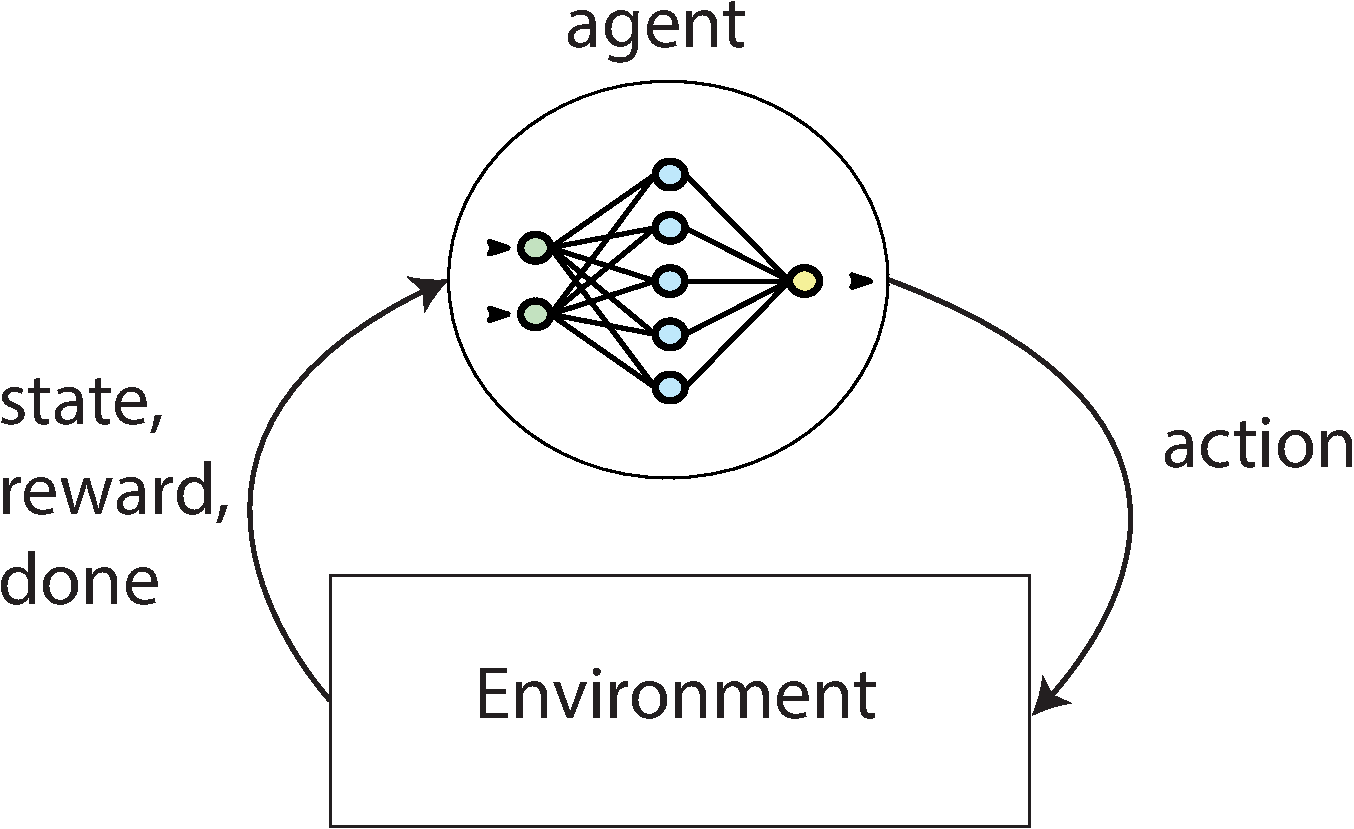
\includegraphics[width=0.6\linewidth]{images/rl_setting}
    }
    \caption{Ваимодействие RL агента и среды}\label{fig:rl_setting}
\end{figure}

Математическое ожидание суммарной дисконтированной награды вычисляется по траекториям при условии текущей стратегии агента по формуле: 

\[
E_{\tau \sim \pi(\theta)} [G(\tau)] = E_{\tau \sim \pi(\theta)} [R_0 + \gamma R_{1} + \gamma ^ 2 R_{2} + ...] = E_{\tau \sim \pi(\theta)} [\sum_{t=0}^{T - 1} \gamma ^t R_{t}]
\]

Взаимодействие агента и среды рассматривается в предположении Марковского процесса принятия решений. Свойство Марковости говорит о том, что следующее состояние среды и получаемая агентом награда зависят только от предыдущего состояния среды и действия совершенного агентом в этом состоянии. 
С учетом этого предположения оптимальная стратегия агента зависит только от текущего состояния среды, что позволяет использовать уравнение оптимальности Беллмана, выражающее связь между оптимальной стратегией в двух последовательных состояниях среды $s$ и $s'$

\[
	V^*(s) = \max_{a \in \mathcal{A}} E(r_{t + 1}(s, a, s') + \gamma V^*(s_{t + 1}))
\]
где $V^*(s)$ (V-функция) - математическое ожидание суммарной дисконтированной награды в состоянии $s$ при условии оптимальной стратегии, а $\gamma$ - коэффициент дисконтирования. Эквивалентно уравнение Беллмана можно записать следующим образом: 

\[
	Q^*(s, a) = E(r_{t + 1}(s, s', a) + \max_{a \in \mathcal{A}} \gamma Q^*(s_{t + 1}, a))
\]
где $Q^*(s, a)$ (Q-функция) - математическое ожидание суммарной дисконтированной награды в состоянии $s$ при условии действия $a$ и следовании оптимальной стратегии в следующем состоянии $s'$.

Далее рассматриваются основные алгоритмы, применяемые в машинном обучении с подкреплением. Условно их можно разделить на два больших класса off-policy и on-policy методы. Off-policy методы основываются на идее аппроксимации Q-функции c использованием метода временных разностей. Такие методы могут использовать данные, полученные стратегией, сколь угодно сильно отличающейся от текущей стратегии. Благодаря этому off-policy методы обычно требуют меньше данных, но более подвержены численным нестабильностям при обучении. С другой стороны, для следующей итерации on-policy методам требуется опыт взаимодействия текущей стратегии со средой благодаря чему они численно более стабильны, но требуют существенно больше данных для обучения. 

%Затем рассматриваются сложности которые возникающие в обучении с подкреплением. Первая из них это \textbf{застревание в локальных оптимумах}. В качестве примера можно представить себе задачу в которой агенту нужно пройти из верхнего левого угла в правый нижний, при этом избегая столкновения со случайно движущимися препятствиями. При столкновении агент получает награду -1, при удачном прохождении +1, при стоянии на месте 0. С большой долей вероятности агент выучит субоптимальную стратегию, которая будет стоять на месте. Следующая сложность состоит в определении того, какие именно действия агента привели к получению награды. Эта проблема носит название \textbf{Credit assignment problem}. 
Затем рассматриваются задачи с \textbf{разреженной наградой}. В таких задачах вероятность того, что агент со случайной стратегией найдет не нулевую награду и тем самым получит положительный сигнал для обучения пренебрежимо мала. В этом случае используются подходы, называемые внутренней мотивацией (intrinsic motivation). Общая идея данных подходов заключается в том, чтобы давать агенту награды за достижение состояний в которых он раньше не был, что позволит эффективно исследовать среду. 
%Последней рассматривается \textbf{дилема исследования-использования} (exploration-exploitation trade-off). В ней идет речь о выборе баланса между исследованием среды и оптимизацией получаемой награды. 
Далее рассматриваются алгоритмы \textbf{мета-обучения}. Обычно, методы обучения с подкреплением предназначены для
решения конкретной задачи и не могут легко обобщаться на другие похожие задачи. Для того чтобы обучить агента решению другой задачи, его обучение
приходится начинать заново. Мета-обучение позволяет агенту выучить такую стратегию, которая сможет адаптироваться к различным задачам. Последним из подходов, используемых в обучении с подкреплением, рассматривается \textbf{иерархическое обучение с подкреплением}. Основная идея иерархического обучения с подкреплением состоит в построении стратегии в виде иерархии навыков, в которой стратегии нижнего уровня решают подзадачи, используемые следующими стратегиями для решения более общих задач. Такое разделение может быть полезным во многих задачах, например в задаче управления шагающим роботом стратегия нижнего уровня отвечает за навык шагать в указанном направлении, а стратегия верхнего уровня использует этот навык для перемещения робота в заданную точку. 

В конце главы рассматривается применение методов глубокого машинного обучения с подкреплением в задачах управления робототехническими устройствами. В последнее время методы RL достигли выдающихся результатов, таких как сборка кубика рубика робо-рукой \cite{rubic} и даже управление термоядерным реактором \cite{tokomak}. По сравнению с методами основанными на классических алгоритмах управления таких как обратная кинематика, алгоритмы машинного обучения способны самостоятельно адаптироваться к параметрам робота и соответственно работать в условиях, когда эти параметры точно не известны или значения, получаемые при измерении этих параметров, имеют большой разброс. 

\underline{\textbf{Вторая глава}} посвящена разработке программно-аппаратного комплекса для настройки оптического интерферометра основанного на машинном обучении с подкреплением.
В начале главы описываются физические принципы работы оптического интерферометра. Работа оптического интерферометра основана на принципе интерференции света - при наложении двух когерентных световых волн возникают осцилляции света различной амплитуды в различных точках пространства. В зависимости от того, происходит наложение волн в синфазно или в противофазе интерференция приводит к увеличению или к уменьшению суммарной амплитуды колебаний. В рамках данной работы рассматривалась интерференция двух световых пучков испущенных одним лазерным источником света. В этом случае интерференционная картина выгладит как череда ярких и темных полос различимых невооруженным взглядом. Схематически интерференционная картина получаемая при наложении двух световых пучков с направлениями заданными волновыми векторами $k1$ и $k2$ изображена на рисунке \ref{fig:two_beam_interf}.

\begin{figure}[ht]
    \centerfloat{
        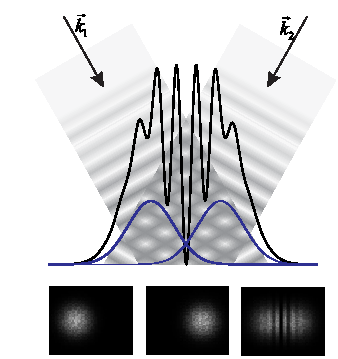
\includegraphics[width=0.5\linewidth]{images/two_beam_inreference.pdf}
    }
    \caption{
     Одномерный срез интерференционной картины полученной при не полном перекрытии двух когерентных лазерных лучей с волновыми векторами ~k1 и ~k2. Фронт волны показан с помощью градиента серого; голубые линии показывают интенсивности каждого пучка (не в масштабе); черная линия показывает интенсивность интерференционной картины. Двумерные интерференционные картины соответствующие одномерному случаю изображены под внизу.}
\label{fig:two_beam_interf}
\end{figure}

В интерферометре принцип интерференции используется для прецизионного измерения относительной разности фаз между двумя когерентными лазерными лучами. Интерферометр является одним из основных инструментов используемых при проведении оптических экспериментов. Например, интерферометр Фабри-Пьеро используется в спектроскопии \cite{fabry-perot1899}; современные детекторы гравитационных волн LIGO и VIRGO \cite{LIGO, VIRGO} используют интерферометр Майкельсона; интерферометр Саньяка используется в системах навигации \cite{Kandpal2000}; интерферометр Маха-Цендера является основным инструментом при проведении современных экспериментов в квантовой оптике \cite{Ourjoumtsev2006, Sychev2017}.

Далее рассмотрим конфигурацию интерферометра Маха-Цендера изображенную на рисунке \ref{fig:interf_scheme_1}. 

\begin{figure}[ht]
    \centering
     \begin{subfigure}[b]{0.45\linewidth}
         \centering
         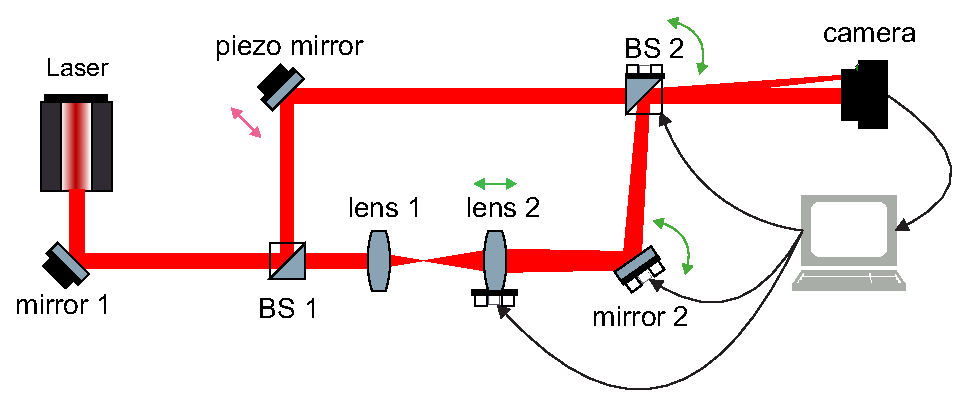
\includegraphics[width=1\linewidth]{interferobot_scheme}
     \end{subfigure}
     \centering
     \begin{subfigure}[b]{0.45\linewidth}
         \centering
         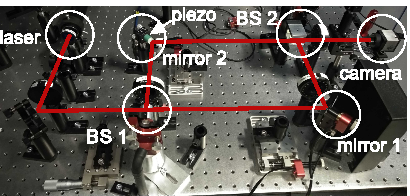
\includegraphics[width=1\linewidth]{interf_real_1}
     \end{subfigure}
    \caption{
     Принципиальная схема и экспериментальная установка интерферометра Маха-Цендера. }
\label{fig:interf_scheme_1}
\end{figure}

На схеме изображенной на рисунке \ref{fig:interf_scheme_1} лазерный луч делится на два первым светоделителем (BS 1). Затем два луча идут по двум плечам интерферометра и объединяются на втором светоделителе (BS 2). Результирующая интерференционная картина снимается с помощью цифровой камеры. Для управления зеркалом (mirror 1) и светоделителем (BS 2) и линзой (lens 2) используются оптомеханические подвижки. Подвижки зеркала и светоделителя могут поворачиваться в двух плоскостях, а подвижка зеркала движется вдоль прямой. Управление производится компьютером с помощью актуатора. Цель настройки интерферометра состоит в том, чтобы точно совместить два пучка после прохождения плеч интерферометра так, чтобы положения их центров, направления k-векторов и кривизна волнового фронта совпали. Настройка интерферометра производится на основе интерференционной картины наблюдаемой на камере. Важной частью наблюдений является временная динамика интерференционных полос наблюдаемая благодаря пьезо зеркалу (mirror 2) которое движется периодически с амплитудой порядка длины волны. В нашем эксперименте время прямого прохода пьезо зеркала больше чем время обратного прохода, что позволяет судить не только об абсолютной величине угла между k-векторами, но и о его знаке. 

Несмотря на кажущуюся простоту, процесс настройки интерферометра довольно трудоемкий. Во-первых, это связано с тем, что каждое движение зеркала  (mirror 1) и светоделителя (BS 2) приводит к одновременному изменению как положения на камере, так и направления нижнего луча. Таким образом при сведении лучей нарушается их параллельность и наоборот. Во-вторых, интерференционная картина получаемая с помощью камеры может содержать шум, оптические аберрации и частицы пыли как показано на рисунке \ref{fig:noise}(a). В третьих оптомеханические подвижки управляющие положениями оптических элементов имеют существенный гистерезис и ограниченную чувствительность.

\begin{figure}
\centering
  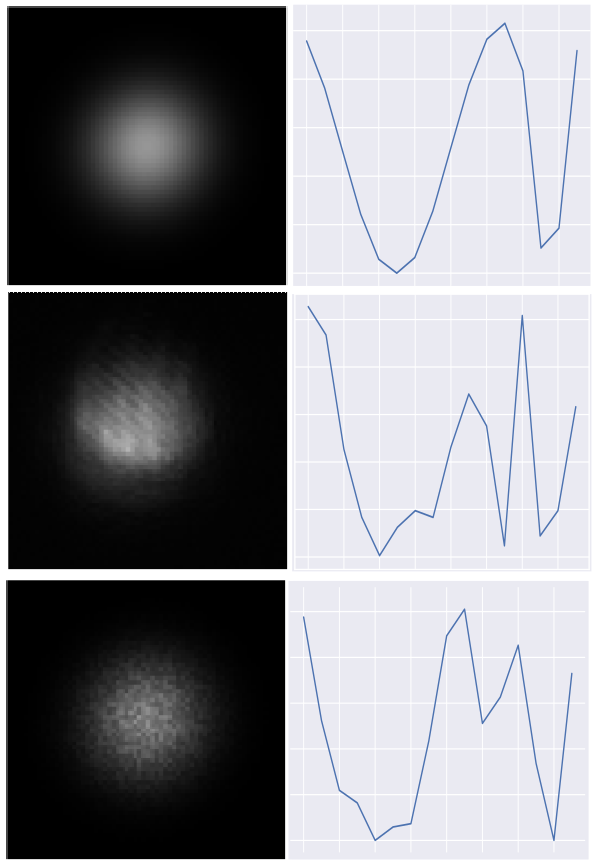
\includegraphics[width=0.5\linewidth]{beamsamples}

\caption{Лазерные лучи: (a) экспериментальный; (b) модель использующая Гауссовый профиль; (c) модель с шумом. На рисунке (a), полосы видны из-за переотражения света от стекла камеры.}
\label{fig:noise}
\end{figure}

Далее приводится построенная на основе этих принципов компьютерная модель позволяющая моделировать изображения, получаемые на камере оптического интерферометра при произвольном расположении оптических элементов - зеркал и линз интерферометра. В нашей модели лазерные лучи в поперечном сечении описываются функцией Гаусса. Вектор напряженности электрического поля в точке $(x,y,z)$ для луча идущего по верхнему плечу интерферометра задается выражением:

\begin{equation}
    E_u={\textrm Re}\left[\exp \left(-\frac{x^{2}+y^{2}}{r_u^{2}(z)}\right) \exp \left(-i\left(k_{z} z+ k\frac{x^2+y^2}{2\rho^2_u(z)} + \phi_{\textrm piezo}(t)\right)\right)\right]
    \label{eq:upper_beam}
\end{equation}

Вектор напряженности электрического поля для луча идущего по нижнему плечу интерферометра:

\begin{multline}
    E_l={\textrm Re}\biggl[\exp \left(-\frac{\left(x-x_{0}\right)^{2}+\left(y-y_{0}\right)^{2}}{r_l^{2}(z)}\right)  \cdot \\
    \exp \left(-i\left(k_{x} x+k_{y} y+k_{z} z + k\frac{x^2+y^2}{2\rho^2_l(z)} z\right)\right)\biggr]
    \label{eq:lower_beam}
\end{multline}

где $(x_0, y_0)$ положение центра нижнего пучка [центр верхнего пучка предполагается в $(x,y)=(0,0)$], луч распространяется вдоль оси $z$ , %$\mathcal N$ the normalization factor, 
$r(z)$ радиус луча, $\rho(z)$ радиус кривизны волнового фронта, $(k_x,k_y,k_z)$ волновой вектор с $k=\sqrt{k_x^2+k_y^2+k_z^2}=2\pi/\lambda$, и $\phi_{\textrm piezo}(t)$ фазовый сдвиг из-за периодического движения пьезо зеркала. В работе используется параксиальное приближение $k_z \gg k_x, k_y$. 

До прохождения светоделителя (BS 1) два луча имеют идентичные параметры. Для вычисления параметров луча после прохождения системы линз используется широко применяемый в оптике формализм ABCD-матриц. В нем луч характеризуется комплексно значным параметром $\dfrac{1}{q} = \dfrac{1}{\rho} - \dfrac{i \lambda}{\pi r^2}$ и изменение параметров луча при прохождении через систему линз записывается следующим образом  $q'=\dfrac{A q+B}{C q+D}$, 
где результирующая матрица системы $M_{total}$ вычисляется как произведение матриц  $M_{total} = M_{lens1} \cdot M_{fs} \cdot M_{lens 2}$
соответствующих распространению луча в пустом пространстве на расстояние $d$, $M_{fs}=\begin{bmatrix} 1 & d \\ 0 & 1 \end{bmatrix}$ и тонкой линзы с фокальным расстоянием $f$  $M_{lens}=\begin{bmatrix} 1 & 0 \\ -1/f & 1 \end{bmatrix}$.

Основной метрикой качества настройки интерферометра является видность интерференционной картины: 

\begin{equation}
    V = \frac{\max_{t}(I_{\textrm tot}) - \min_t(I_{\textrm tot})
            } {
                \max_{t}(I_{\textrm tot}) + \min_t(I_{\textrm tot})
            },
    \label{eq:visib}
\end{equation}

где $I_{\textrm tot}(t) = \iint_{-\infty}^{+\infty} I(x, y, t) {\textrm d}x{\textrm d}y$ суммарный световой поток падающий на камеру; максимум и минимум вычисляются за один проход пьезо зеркала. Видность по определению лежит в интервале от 0 до 1. Для полностью настроенного интерферометра [рисунок~\ref{fig:visib_expl}(a)], $\min_t(I_{\textrm tot})=0$, таким образом $V=1$, для полностью расстроенного интерферометра [рисунок~\ref{fig:visib_expl}(c)], $\min_t(I_{\textrm tot})\approx\max_t(I_{\textrm tot})$, таким образом $V\approx 0$.

Мы моделируем матрицу камеры в виде эквидистантной сетки $64\times64$ пикселя и вычисляем интенсивность света в каждом пикселе. Камера располагается в точке $(x,y)=(0,0)$, таким образом луч проходящий через верхнее плечо интерферометра попадает в центр камеры. На каждый проход пьезо зеркала мы моделируем 16 интерференционных картин соответствующих различным  $\phi_{\mathrm{piezo}}(t)$. Мы вычисляем видность интерференционной картины в соответствии с уравнением~\ref{eq:visib}. Так как для успешного обучения RL-агентов требуются миллионы взаимодействий со средой мы реализовали симулятор на C++, а вычисления интенсивности производим параллельно. Итоговая скорость работы симулятора на процессоре intel core i7 составила более 200 фреймов, состоящих из 16 изображений, в секунду. Для обучения агентов симулятор имеет стандартный gym интерфейс. 

Примеры изображений полученных с помощью разработанной программы приведены на рисунке \ref{fig:visib_expl}. 

\begin{figure}[ht]
    \centerfloat{
        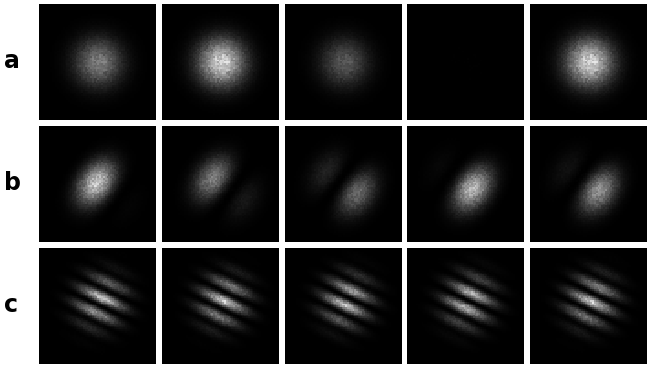
\includegraphics[width=0.8\linewidth]{images/visib_expl}
    }
    \caption{
    Изображения интерференции для различных положения зеркал полученные с помощью симуляционной программы. (a) Идеально настроенный интерферометр, видность = 1; (b) Слабо расстроенный интерферометр, видность = 0.3; (c) Сильно расстроенный интерферометр, видность = 0.0026. Изображения слева на право соответствуют различным моментам времени.}
\label{fig:visib_expl}
\end{figure}

Геометрические размеры интерферометра использованные при моделировании и при проведении экспериментов приведены в таблице \ref{tab:interf_stat_params}. Фокусные расстояния линз lens1 и lens2 равны 50 мм. В настроенном состоянии интерферометра расстояние между линзами равно сумме фокусных расстояний. Линза lens 1 располагается на расстоянии 50 мм от светоделителя BS 1.  

\begin{table} [htbp]
    \centering
    \begin{threeparttable}% выравнивание подписи по границам таблицы
        \caption{Параметры интерферометра, мм}
        \begin{tabular}{|c|c|c|c|c|}
            \hline
            \hline
            параметр   & длина & ширина & расстояние до камеры & радиус пучка \\
            \hline
            значение & 200 & 300 & 100 & 0.71 \\
            \hline
            \hline
        \end{tabular}
        \label{tab:interf_stat_params}
    \end{threeparttable}
\end{table}

Максимальные смещения от настроенного положения для оптических элементов приведены в таблице \ref{tab:interf_dyn_params}. Значения подбирались так, чтобы наблюдать весь спектр интерференционных картин наблюдаемых в эксперименте.

\begin{table} [htbp]
    \centering
    \begin{threeparttable}% выравнивание подписи по границам таблицы
        \caption{Максимальное значение смещения каждого оптического элемента. Углы зеркал в радианах, положения линз в миллиметрах.}
        \begin{tabular}{|c|c|c|c|c|c|}
            \hline
            \hline
            параметр & mirror 2, x & mirror 2, y & BS 2, x & BS 2, y & lens 2 \\
            \hline
            значение & $2.6 \cdot 10^{-3}$ & $1.8 \cdot 10^{-3}$ & $1.3 \cdot 10^{-3}$ & $0.9 \cdot 10^{-3}$ & $7.5$ \\
            \hline
            \hline
        \end{tabular}
        \label{tab:interf_dyn_params}
    \end{threeparttable}
\end{table}


Далее формулируется задача настройки интерферометра в терминах машинного обучения с подкреплением, приводятся результаты обучения агентов использующих непрерывное и дискретное пространство действий и результаты тестирования обученных агентов на экспериментальной установке. 

Мы сводим процесс настройки интерферометра к Марковскому процессу принятия решений. Состоянием среды $s$ является последовательность из 16 интерференционных изображений полученных за 1 проход пьезо зеркала. Действия агента должны управлять положением оптических элементов линз и зеркал интерферометра. Для этого мы рассматриваем два способа задания пространства действий - дискретное и непрерывное. В случае дискретного пространства действий агент может оперировать заданным заранее набором длин шагов. В нашей реализации агент может менять положения оптических элементов независимо и только по одному направлению за раз. Это позволяет агенту с одинаковой уверенностью использовать шаги как большой, так и маленькой амплитуды. Для обучения агента использовался алгоритм DQN \cite{dqn}.  Однако такой способ требует ручного задания дискретизации и ограничивает количество оптических элементов которыми агент может оперировать одновременно. Настройки интерферометра с использованием непрерывного пространства действий позволяет решить эти проблемы. В этом случае агент может оперировать одновременно всеми оптическими элементами и изменять их положение на произвольную величину. Действие $a$ представляет собой N-мерный вектор $a \in (-1, 1)^{N}$. 
В этом случае для обучения агента использовался алгоритм TD3 \cite{ddpg}.
Так как в конце настройки интерферометра действия агента становятся на два порядка меньше чем в начале мы применяем ренормировку действий следующим образом: 

\begin{equation}
a =
   \begin{cases}
    {\textrm sign}(a) \cdot 1000^{|a| - 1}  & \quad \text{if $|a| > 0.17$} 
    \\
    0  & \quad \text{if $|a| \leq 0.17$}
  \end{cases}
\end{equation}
Такая ренормировка приводит к действиям в интервале $|a|\in\{0\}\cup[2.5 \cdot 10^{-3}, 1]$.

Далее обосновывается выбор функции награды. Видность интерференции $V$ не является хорошей наградой, так как она не позволяет агенту достоверно различать состояния с видностью вблизи 1, что важно при проведении экспериментов. Была выбрана функция награды $r = V - \log(1 - V)$, где V - видность интерференционной картины. С такой функцией награды агент получает награду не только в начале, но и в конце эпизода когда видность близка к 1. 

Для того чтобы обученного в симуляции агента можно было применять на экспериментальной установке при обучении использовались рандомизации среды основанные на неопределенности параметров установки. В начале каждого эпизода мы случайно изменяли радиус луча на ±20\%, так как этот параметр сложно точно измерить. Изменение радиуса также помогает бороться с отклонением профиля экспериментального луча от распределения Гаусса. Следующие рандомизации использовались на каждом шаге. Во-первых, мы случайно изменяли яркость интерференционной картины на ±30\%, что моделирует различное время выдержки камеры. Во вторых мы добавили 20\% белого шума в каждый пиксел изображения, что можно рассматривать как шум камеры, так и как наличие пыли на камере \ref{fig:noise}. В третьих мы добавили циклический сдвиг интерференционных изображений полученных за один проход пьезо зеркала и рандомизировали соотношение времен прямого и обратного проходов пьезо зеркала. Отношение числа изображений полученных во время прямого прохода было больше чем 50\%. 

\begin{figure}[ht]
    \centerfloat{
        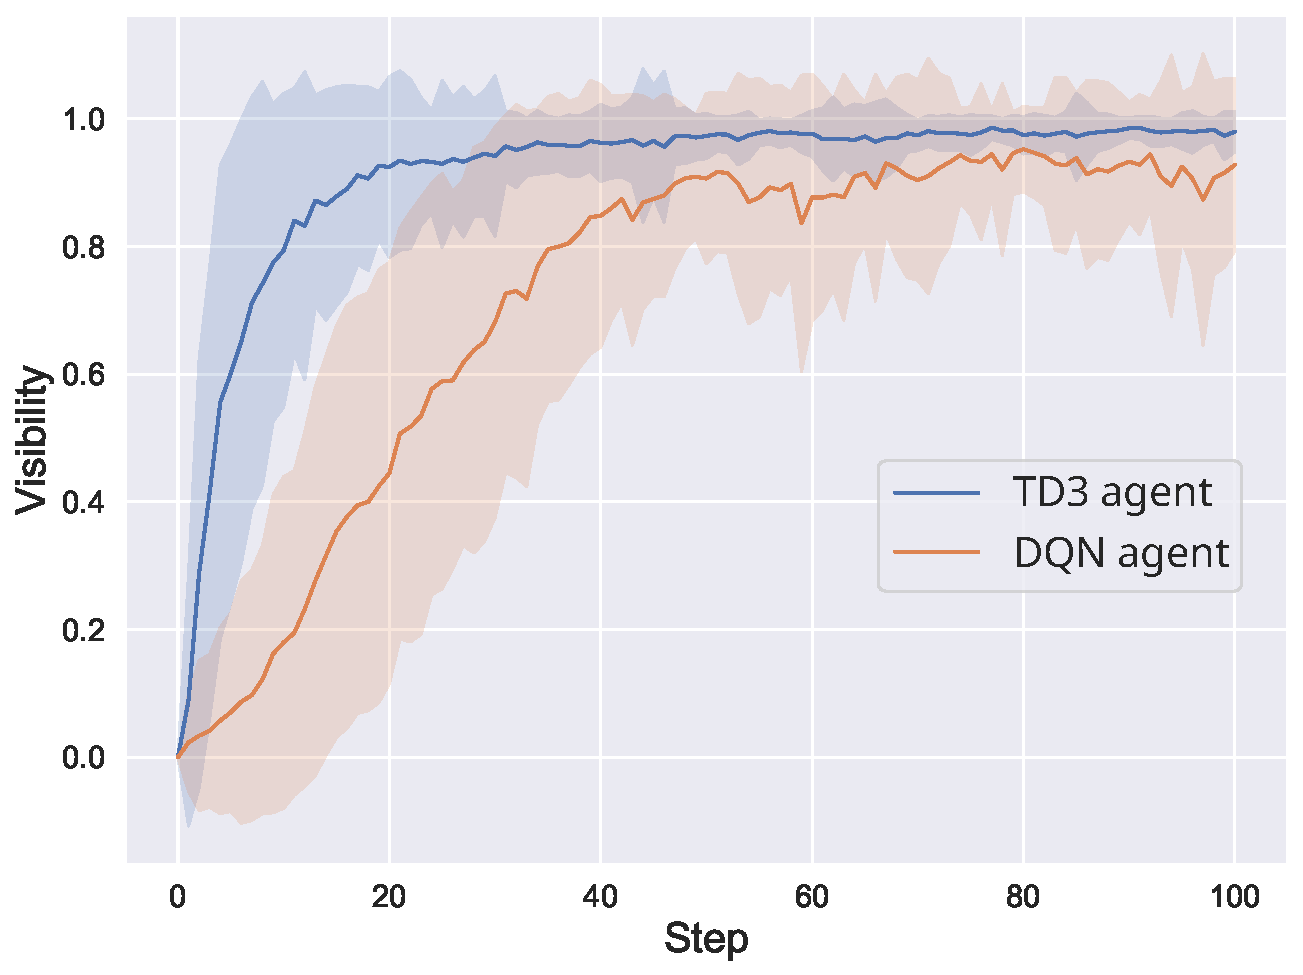
\includegraphics[width=0.8\linewidth]{images/dqn_vs_td3}
    }
    \caption{Тестирование агентов на экспериментальной установке}\label{fig:interf_test}
\end{figure}

В заключении главы описываются основные характеристики программно-аппаратного комплекса предназначенного для тестирования обученного агента на экспериментальной установке; приводятся результаты тестирования агентов на экспериментальной установке; приводится сравнение качества настройки интерферометра с человеком и анализ стратегии, используемой агентами при настройке интерферометра. Результаты тестирования приведены на рисунке \ref{fig:interf_test}. По оси абсцисс отложен номер шага настройки, по оси ординат отложена достигнутая видность. Результаты усреднены по 100 эпизодам. Из рисунка \ref{fig:interf_test} видно, что оба метода достигают хорошего значения видности интерференционной картины, но агент TD3 использующий непрерывное пространство действий работает быстрее и достигает лучшей видности чем DQN агент использующий дискретное пространство действий. 

Результаты сравнения качества настройки интерферометра разработанным методом с экспертом приведены в таблице \ref{tab:human}. Из нее видно, что агент использующий дискретное пространство действий работает на уровне человека как по качеству настройки, так и по скорости. TD3-агент использующий непрерывное пространство действий настраивает интерферометр существенно лучше, чем человек. 

\begin{table} [htbp]
    \centering
    \begin{threeparttable}
        \caption{Сравнение разработанных методов с экспертом. В таблице приведено время требуемое для достижения видности интерференции 0.92, 0.95 и 0.98. Также в скобках приведен процент эпизодов когда эта видность не достигнута.}
        \label{tab:human}
        \begin{tabular}{| p{2.5cm} || p{2.5cm} | p{2.5cm} | p{2.5cm} |}
            \hline
            \hline
            &V $\ge 0.92$ & V $\ge 0.95$ & V $\ge 0.98$\\
            \hline
            Эксперт &  93.9 (\textbf{0\%})  & 103.6 (\textbf{0\%}) & 129.6 (10\%)\\
            TD3 &  \textbf{56.16} (\textbf{0\%}) & \textbf{75.06} (\textbf{0\%}) & \textbf{120.1} (\textbf{4\%})\\
            DQN &  98.7 (7.6\%) & 116.1 (7.6\%) & 156.4 (10.6\%)\\
            \hline
            \hline
        \end{tabular}
    \end{threeparttable}
\end{table}

Результаты работы опубликованы в статьях \cite{confbib1, confbib2} на ведущих научных конференциях <<Neural information processing systems (NeurIPS)>> и <<Conference on Robot Learning (CoRL)>> также на программу автоматической настройки интерферометра по изображениям с камеры с использованием машинного обучения получен РИД \cite{progbib1}.

\underline{\textbf{Третья глава}} посвящена исследованию методов машинного обучения с подкреплением для использования в среде Nethack. Среда Nethack основана на одноименной игре и предложена в качестве теста для алгоритмов машинного обучения в 2020 году \cite{nethack}. В этой игре агент путешествует по процедурно генерируемому подземелью. Игра имеет ascii интерфейс изображенный на рисунке \ref{fig:nethack}.

\begin{figure}[ht]
    \centerfloat{
        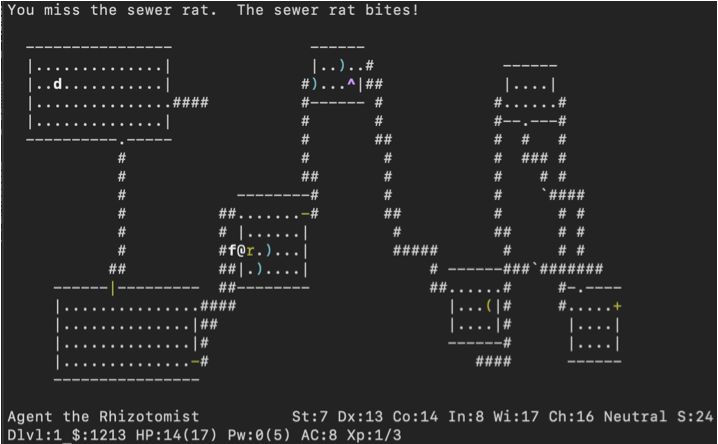
\includegraphics[width=0.8\linewidth]{images/nethack}
    }
    \caption{Игра Nethack}\label{fig:nethack}
\end{figure}

Основную сложность для алгоритмов обучения с подкреплением составляют сочетание различных типов данных в состоянии (изображения, текстовые описания, табличные данные), редкая функция награды и комбинаторно большое пространство действий. Для решения этой задачи нами был разработанный метод, сочетающий в себе машинное обучение с подкреплением, алгоритмы навигации на графах и алгоритмы, основанные на экспертных знаниях \ref{alg:raph}. Для решения различных подзадач возникающих в процесс игры таких как сражение с монстрами, исследование подземелья, обращение с предметами нами была реализована отдельная стратегия. Выбор стратегии на каждом шаге происходил в соответствии с их приоритетом заданным вручную. Стратегия сражения с монстрами обучалась с помощью алгоритма IMPALA \cite{impala} и имела дискретное пространство действий. Остальные стратегии были реализованы с использованием алгоритмов навигации на графах. Данный подход позволил превзойти остальные подходы с использованием обучения с подкреплением в этой задаче. Результаты были опубликованы на одной из ведущих конференции по машинному обучению NeurIPS в рамках трека посвященного соревнованиям \cite{confbib3}.


\begin{algorithm}[ht]
\SetKwComment{Comment}{/* }{ */}
\SetKw{Continue}{continue}
\caption{RAPH agent}\label{alg:raph}
\KwData{view\_distance, agent, hard\_coded\_skills}
$state, done \gets env.reset(), False$\;

\While{not done}{
  action\_queue = parse\_message(state)\;

  \If{action\_queue} {
   state, reward, done, info = env.step(action\_queue)\Comment*[r]{We have a prompt to response}
   \Continue
  }

  monster\_distance, preprocessed\_state = parse\_dungeon(state)\;
  \eIf{monster\_distance \textless view\_distance}{
    action\_queue = agent.act(preprocessed\_state)\;
  }{
    action\_queue = first\_fit(hard\_coded\_skills, preprocessed\_state)\Comment*[r]{Select non-rl action on first-fit basis}
  }
  state, reward, done, info = env.step(action\_queue)\;
}
\end{algorithm}

\underline{\textbf{Четвертая глава}} посвящена разработке метода основанного на обучении с подкреплением для управления движением
робота Unitree A1~\cite{unitree}. Для обучения стратегии была разработана функция награды
которая побуждает агента выучивать безопасное и плавное движение с заданной скоростью. Обучение и тестирование агента производилось в симуляции с использованием симулятора Raisim \cite{raisim}. Обучение агента производилось с помощью алгоритма PPO~\cite{Schulman2017ProximalPO}. Для того чтобы агент выучил устойчивую стратегию во время
обучения в наблюдения добавлялись шумы и на робота воздействовала сила в случайном направлении. Пространство состояний включало в себя информацию об ориентации, скорости робота, а также положения и скорости его суставов. Пространство действий было непрерывным и каждое действие соответствовало желаемому положению составов робота. Результаты тестирования приведены в таб.~\ref{tab:unitree_eval} и на рис.~ \ref{fig:unitree_eval_forward}. В таблице \ref{tab:unitree_eval} приведены результаты тестирования обученного агента для задач ``Движение вперед'', ``Движение назад'', ``Поворот по часовой стрелке'' и ``Поворот против часовой стрелки''. Видно, что для задач ``Движение вперед'', ``Движение назад'' стратегия более стабильна и число шагов близко к максимальной длине эпизода. В задачах ``Поворот по часовой стрелке'' и ``Поворот против часовой стрелки'' выученная стратегия менее стабильна, что приводит к меньшей суммарной награде и меньшему среднему числу шагов. Причиной этому может служить то, что случайная сила прикладываемая во время обучения и во время тестирования для обучения устойчивой стратегии дестабилизирует поворачивающегося агента больше чем движущегося прямо.

\begin{figure}[h]
\begin{subfigure}{.5\textwidth}
  \centering
  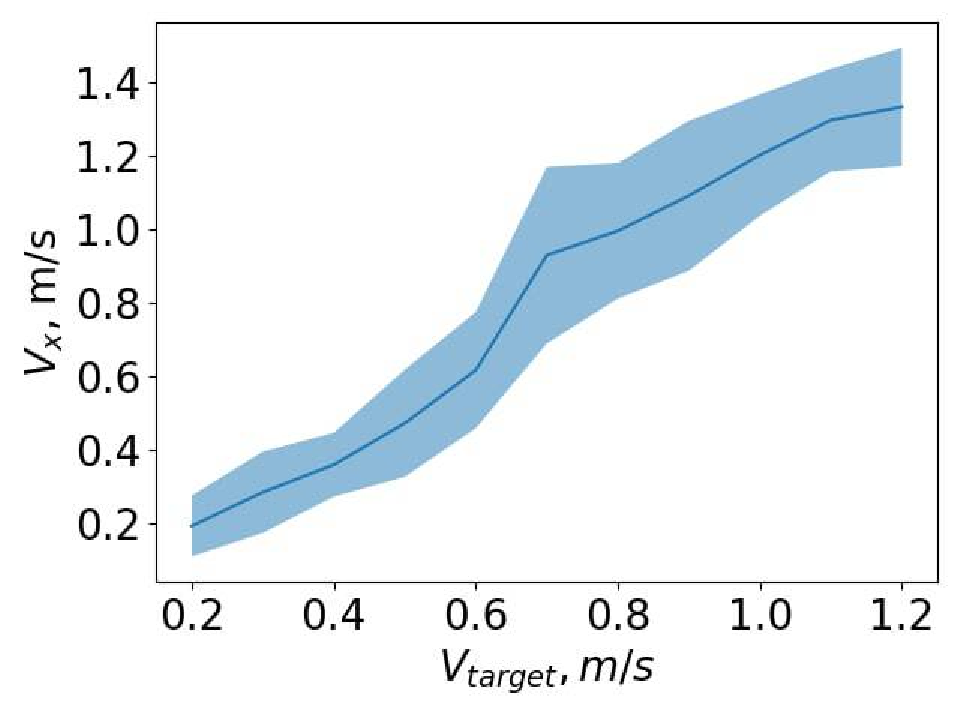
\includegraphics[width=1\textwidth]{images/vx}
\end{subfigure}%
\begin{subfigure}{.5\textwidth}
  \centering
  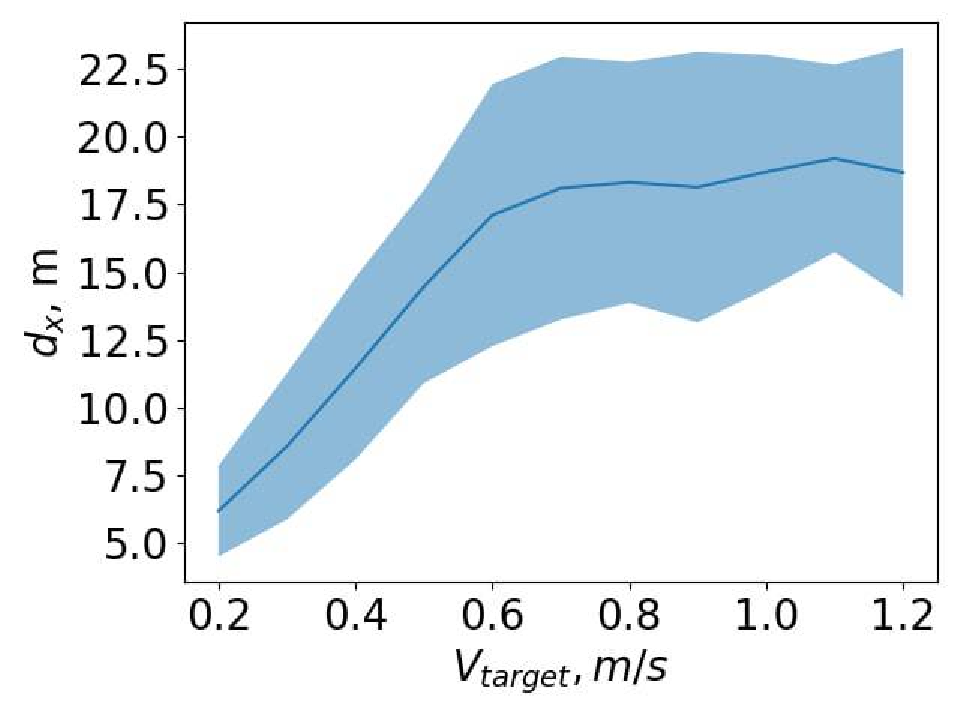
\includegraphics[width=1\textwidth]{images/dx}
\end{subfigure}%
\caption{Тестирование задачи ``Движение вперед с заданной скоростью''. (a) Скорость робота $V_x$ как функция целевой скорости $V_{target}$. (b) Расстояние пройденное роботом к концу эпизода $d_x$ как функция целевой скорости $V_{target}$.}
\label{fig:unitree_eval_forward}
\end{figure}

На рис.~\ref{fig:unitree_eval_forward} представлены результаты тестирования обученной стратегии в задаче ``Движение вперед с заданной скоростью''. Из рис.~\ref{fig:unitree_eval_forward}a видно, что обученный агент способен двигаться с различной скоростью и его скорость близка к целевой скорости. Расстояние пройденное агентом вдоль оси $x$ показано на рис.~\ref{fig:unitree_eval_forward}b. При целевой скорости $V_{target} \in$ (0, 0.6) м/с расстояние пройденное к концу эпизода растет. При целевой скорости больше 0.6 м/с пройденное расстояние практически постоянно и равно расстоянию от агента до края среды.

\begin{table} [htbp]
    \centering
    \begin{threeparttable}
        \caption{Результаты тестирования обученного агента в симуляции}\label{tab:unitree_eval}
        \begin{tabular}{| p{2cm} || p{2cm} | p{2cm} | p{2cm} |p{2cm} |}
            \hline
            \hline
            Задача & Движение вперед & Движение назад & Поворот по часовой стрелке & Поворот против часовой стрелки \\
            \hline
            Суммарная награда &	529 $\pm$ 124 &	508 $\pm$ 98 &	85 $\pm$ 219 &	165 $\pm$ 155 \\
            Число шагов & 3263 $\pm$ 633 &	3136 $\pm$ 545 &	2057 $\pm$ 1208 &	2095 $\pm$ 1325 \\
            \hline
            \hline
        \end{tabular}
    \end{threeparttable}
\end{table}

Полученные результаты показывают, что линейной и угловой скоростью робота Unitree A1 с хорошим качеством можно управлять с помощью обучения с подкреплением. 



\FloatBarrier
\pdfbookmark{Заключение}{conclusion}                                  % Закладка pdf
В \underline{\textbf{заключении}} приведены основные результаты работы, которые заключаются в следующем:
%% Согласно ГОСТ Р 7.0.11-2011:
%% 5.3.3 В заключении диссертации излагают итоги выполненного исследования, рекомендации, перспективы дальнейшей разработки темы.
%% 9.2.3 В заключении автореферата диссертации излагают итоги данного исследования, рекомендации и перспективы дальнейшей разработки темы.
\begin{enumerate}
  \item Была разработанна компьютерная модель оптического интерферометра Маха-Цендера. Процесс настройки интерферометра был представлен в виде марковского процесса принятия решений на основании которого была разработана среда для обучения агентов машинного обучения с подкреплением по настройке оптического интерферометра. 
  \item На основе среды были разработаны методы основанные на обучении с подкреплением, которые позволили выучить алгоритм настройки интерферометра по изображениям с камеры. 
  \item Разработанные методы были успешно протестированы при настройке экспериментальной установки интерферометра. 
  \item Был разработан метод включающий в себя обучения с подкреплением для управлением виртуальным агентом в среде Nethack. 
\end{enumerate}

\newpage


\pdfbookmark{Литература}{bibliography}                                % Закладка pdf

\ifdefmacro{\microtypesetup}{\microtypesetup{protrusion=false}}{} % не рекомендуется применять пакет микротипографики к автоматически генерируемому списку литературы
\urlstyle{rm}                               % ссылки URL обычным шрифтом
\ifnumequal{\value{bibliosel}}{0}{% Встроенная реализация с загрузкой файла через движок bibtex8
    \renewcommand{\bibname}{\large \bibtitleauthor}
    \nocite{*}
    \insertbiblioauthor           % Подключаем Bib-базы
    %\insertbiblioexternal   % !!! bibtex не умеет работать с несколькими библиографиями !!!
}{% Реализация пакетом biblatex через движок biber
    % Цитирования.
    %  * Порядок перечисления определяет порядок в библиографии (только внутри подраздела, если `\insertbiblioauthorgrouped`).
    %  * Если не соблюдать порядок "как для \printbibliography", нумерация в `\insertbiblioauthor` будет кривой.
    %  * Если цитировать каждый источник отдельной командой --- найти некоторые ошибки будет проще.
    %
    
    \expandafter\def\csname blx@maxbibnames\endcsname{99}% sorokin set et.al max names
    
    %% authorvak
    \nocite{vakbib1}%
    \nocite{vakbib2}%
    %
    %% authorwos
    \nocite{wosbib1}%
    %
    %% authorscopus
    \nocite{scbib1}%
    %
    %% authorpathent
    \nocite{patbib1}%
    %
    %% authorprogram
    \nocite{progbib1}%
    %
    %% authorconf
    \nocite{confbib1}%
    \nocite{confbib2}%
    \nocite{confbib3}%
    \nocite{confbib4}%
    %
    %% authorother
    \nocite{bib1}%
    \nocite{bib2}%

    \ifnumgreater{\value{usefootcite}}{0}{
        \begin{refcontext}[labelprefix={}]
            \ifnum \value{bibgrouped}>0
                \insertbiblioauthorgrouped    % Вывод всех работ автора, сгруппированных по источникам
            \else
                \insertbiblioauthor      % Вывод всех работ автора
            \fi
        \end{refcontext}
    }{
        \ifnum \totvalue{citeexternal}>0
            \begin{refcontext}[labelprefix=A]
                \ifnum \value{bibgrouped}>0
                    \insertbiblioauthorgrouped    % Вывод всех работ автора, сгруппированных по источникам
                \else
                    \insertbiblioauthor      % Вывод всех работ автора
                \fi
            \end{refcontext}
        \else
            \ifnum \value{bibgrouped}>0
                \insertbiblioauthorgrouped    % Вывод всех работ автора, сгруппированных по источникам
            \else
                \insertbiblioauthor      % Вывод всех работ автора
            \fi
        \fi
        %  \insertbiblioauthorimportant  % Вывод наиболее значимых работ автора (определяется в файле characteristic во второй section)
        
        \expandafter\def\csname blx@maxbibnames\endcsname{3}% sorokin reset et.al max names

        \begin{refcontext}[labelprefix={}]
            \insertbiblioexternal            % Вывод списка литературы, на которую ссылались в тексте автореферата
        \end{refcontext}
        % Невидимый библиографический список для подсчёта количества внешних публикаций
        % Используется, чтобы убрать приставку "А" у работ автора, если в автореферате нет
        % цитирований внешних источников.
        \printbibliography[heading=nobibheading, section=0, env=countexternal, keyword=biblioexternal, resetnumbers=true]%
    }
}
\ifdefmacro{\microtypesetup}{\microtypesetup{protrusion=true}}{}
\urlstyle{tt}                               % возвращаем установки шрифта ссылок URL
